%%%% Course preprint. Formatted with the IJCAI--ECAI--26 author kit.
%%%% This work has not been submitted to IJCAI or to any other venue, and no
%%%% claim of acceptance is made or implied. See the footnote on page 1.

\documentclass{article}
\pdfpagewidth=8.5in
\pdfpageheight=11in

\usepackage{ijcai26}

\usepackage{times}
\usepackage{soul}
\usepackage{url}
\usepackage[hidelinks]{hyperref}
\usepackage[utf8]{inputenc}
\usepackage[small]{caption}
\usepackage{graphicx}
\usepackage{booktabs}
\usepackage{amsmath}
\usepackage{amssymb}
\usepackage{multirow}
\urlstyle{same}

\title{Costing How an NPC Reads: Attributability as a Proxy for
Believable Search Behaviour}

\author{
Aqeeb Rizwan\\
\affiliations
Independent\\
\emails
\url{https://github.com/SL-A-SH/AI-Native-Cohort}
}

\begin{document}

\maketitle

\begin{abstract}
A non-player character searching for a hidden player must act on a belief rather than on
knowledge. Occupancy-map methods for this are established in game AI. We take that machinery as
given and ask a narrower question: can the way behaviour \emph{reads} to an observer be priced
as a cost, alongside the tactical costs an agent already pays? We define three such terms
(illegibility, redundancy, dither) and an \emph{attributability} measure computed by running a
second belief that receives no positive observations and comparing the two. On a single
hand-made grid, across 8 case-generation seeds and 40 scenarios each, the resulting agent is
beaten on capture rate by two much cheaper scripted policies in every seed, while re-searching
already-cleared ground roughly a tenth as often. A factorial ablation shows that the
negative-information update and a hand-coded anti-redundancy memory are substitutes rather than
complements: either alone produces most of the effect, and the hand-coded version produces the
best redundancy figure and the worst capture rate. We report these results as an engineering
study. We do not claim that attributability measures believability: no human has judged this
agent, and validating the measure against observer judgement is the experiment the work most
needs.
\end{abstract}

\section{Introduction}

An enemy that always knows where you are is not difficult, it is unpleasant.\footnote{This is a
course preprint, prepared as coursework and formatted with the IJCAI--ECAI--26 author kit. It
has not been submitted to IJCAI or to any other venue, and no claim of review or acceptance is
made.} An enemy that never finds you is not fair, it is broken. Between those two failures sits
the behaviour designers actually want, and it is usually produced by hand.

This paper concerns one narrow part of that problem. Given an NPC that maintains a probability
distribution over a hidden player's location and chooses actions by minimising expected cost, we
ask whether the \emph{legibility} of its choices can be priced in the same objective as its
tactical costs, rather than being left to animation and scripting.

\paragraph{A retracted motivation.}
This work began from a claim that turned out to be false, and we state it plainly because the
correction shapes everything that follows. We believed that shipped game AI represented belief
only discretely, as a remembered position plus an awareness level, and that probabilistic
occupancy methods lived in robotics. That is wrong. Isla introduced occupancy maps to a game AI
audience two decades ago~\cite{isla2006occupancy} and later shipped a commercial stealth game
built around them~\cite{isla2013thirdeye}. The grid, the diffusion over walkable space, and
cell-scope negative information are prior art in games, not a transfer from robotics.

What remains is narrower. The belief machinery here is a replication. The contribution, such as
it is, is the cost layer over it and the attributability measure, both evaluated honestly and
both reported with negative results where we found them.

\paragraph{Contributions.}
\begin{enumerate}
\item A cost formulation with three terms that price how behaviour reads rather than how
accurate it is, each traceable to a specific practitioner complaint (Section~\ref{sec:agent}).
\item An attributability measure: the ratio between the agent's belief and a counterfactual
belief deprived of positive observations (Section~\ref{sec:model}).
\item An evaluation against three controls in which the proposed agent loses on the primary
task, and a factorial ablation showing that its clearest advantage is not caused by the
mechanism we assumed (Sections~\ref{sec:results} and~\ref{sec:failures}).
\end{enumerate}

\section{Related Work and User Discussions}

\paragraph{Belief in shipped game AI.}
Isla's Halo~2 work describes a discrete model: a remembered target position and orientation
plus awareness levels, with the actor explicitly permitted to believe things that are not
true~\cite{isla2005halo2}. F.E.A.R.'s published AI work is goal-oriented action
planning~\cite{orkin2006fear}. The \emph{Alien: Isolation} director holds the player's true
position and deliberately tells the alien only a general area~\cite{tommy2017alien}. Against
these, Isla's occupancy-map work~\cite{isla2006occupancy,isla2013thirdeye} is the direct
antecedent of the belief model used here. The underlying filter is standard recursive state
estimation~\cite{thrun2005probabilistic}.

\paragraph{User discussions.}
Three of the design decisions in this paper came from public discussion with practitioners and
players rather than from literature, and we record which.

A roguelike developer described a shipped give-up rule in his own game: a monster follows the
player into a room, and \textit{``if that room has two doors and I exit, it will give up after it
sees the room empty.''} This retracted our assumption that negative information is generally
absent from game AI. The distinction that survives is narrower and is what we implement: their
rule is \emph{room-scope} and terminates a pursuit, ours is \emph{cell-scope} and redistributes
probability.

A player observed that an omniscient enemy is acceptable when the fiction explains it --- a
mind-reader may know where you are --- while an ordinary guard doing the same thing is
infuriating. Identical information, opposite reaction. This reframed our objective: the
complaint is not about how much the NPC knows but about whether an observer can attribute the
knowledge to something. The attributability measure is our attempt to make that computable.

A second developer noted that his monsters enter a ``where did they go?'' state in which they
look around and pace back and forth to show confusion, before returning to patrol. We had
recorded that oscillation as our worst failure mode; he animates it deliberately. The failure
is therefore not oscillation but oscillation that is unbounded and unexplained.

\section{Agent Design}
\label{sec:agent}

\paragraph{Problem.}
The agent observes a stream of noisy perception events (a sighting, a sound, a door state
change) and the time elapsed since each. It must choose an action because the player's position
is not known.

\paragraph{Input and hidden state.}
The hidden state is the player's cell on a $24\times14$ grid with 201 walkable cells. The agent
never receives the player's position. Its inputs are observations and its own location.

\paragraph{Actions.}
Six: \textsc{search} a cell, \textsc{hold\_position}, \textsc{flank} to a chokepoint,
\textsc{call\_reinforcements}, \textsc{retreat}, and \textsc{resume\_post}, the only terminal
action. Two of these are never chosen in our experiments and we report that as a finding rather
than trimming the action set (Section~\ref{sec:limits}).

\paragraph{Cost terms.}
Each option's cost is a sum. Three terms are tactical: travel, a per-tick cost of the player
remaining at large, and an expected gain crediting belief mass brought under observation. Three
price how the behaviour reads:

\begin{description}
\item[Illegibility] penalises acting where the agent's own evidence does not point, scaled by
the unattributable fraction defined in Section~\ref{sec:model}.
\item[Redundancy] penalises returning to ground swept within the last 25 ticks, decaying with
age. This is a behavioural memory, deliberately separate from the belief.
\item[Dither] penalises abandoning a target before arriving at it.
\end{description}

\paragraph{Human reasoning function.}
The agent identifies its own uncertainty: holding and standing down are priced like every other
option, so ``I do not know enough to commit'' emerges from the comparison rather than from a
tuned entropy threshold.

\paragraph{A caution on the weights.}
The three believability weights are 6, 8 and 4. They are assumed, not fitted. They are also not
independently meaningful: a constant lookahead multiplier scales the gain terms but not travel,
dither or redundancy, so only ratios among the coefficients affect decisions. We report
sensitivity rather than defending the values.

\section{Probability Model and Decision Rule}
\label{sec:model}

The belief $b_t$ over cells alternates predict and update. Prediction diffuses mass to walkable
neighbours, so probability flows around walls rather than through them:
\begin{equation}
b_{t}^{-}(x) = \alpha\, b_{t-1}(x)
 + (1-\alpha) \!\!\sum_{x' \in N(x)} \!\! \frac{w(x)}{\sum_{y \in N(x')} w(y)}\, b_{t-1}(x'),
\end{equation}
with $\alpha = 0.55$ the probability of not moving and $w$ a transition weight (uniform in
policy~A; raised on chokepoints in policy~B). Update is Bayes' rule with an unnormalised
likelihood:
\begin{equation}
b_t(x) \;=\; \frac{L(z_t \mid x)\, b_t^{-}(x)}{\sum_{x'} L(z_t \mid x')\, b_t^{-}(x')}.
\end{equation}
A sighting uses a tight Gaussian about the reported cell, a sound a wider one, both with a
false-positive floor, and distance is measured \emph{through} the map rather than across it. A
failed search multiplies each searched cell by a miss rate of $0.15$, so looking and seeing
nothing reduces a cell without eliminating it.

\paragraph{Attributability.}
Alongside $b_t$ we run $b^0_t$, the same filter receiving diffusion and failed searches but no
positive observations. Their ratio
\begin{equation}
r_t(x) \;=\; b_t(x) \,/\, b^0_t(x)
\end{equation}
is $1$ where the agent would have believed as much anyway. The illegibility term is priced off
$1/r$, capped at $3$.

\begin{figure}[t]
\centering
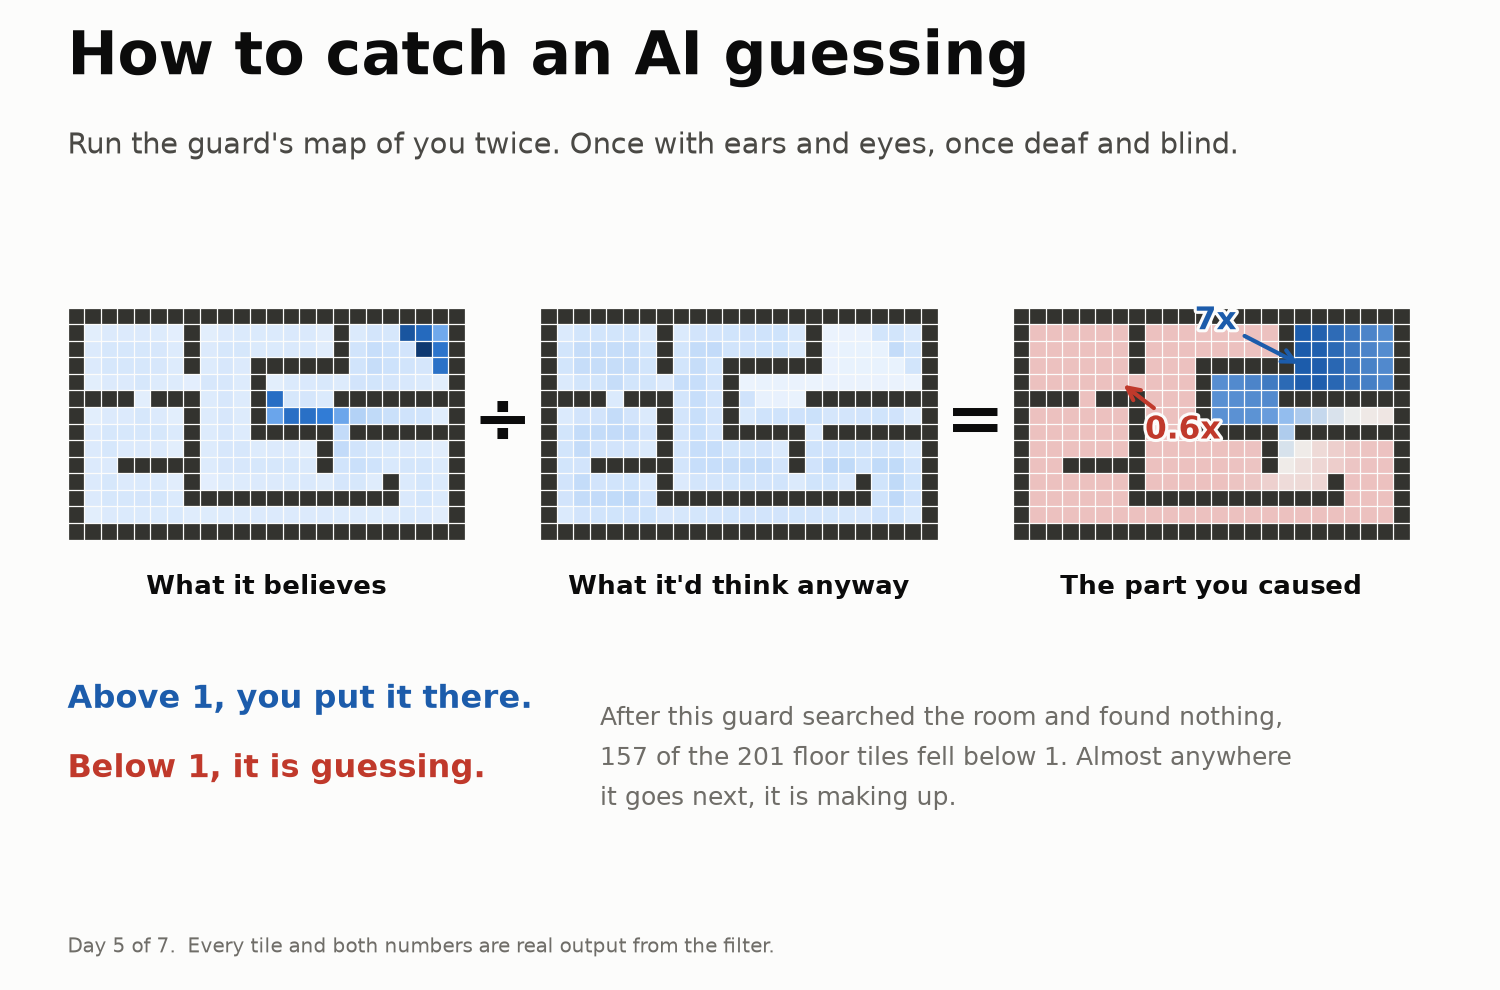
\includegraphics[width=\columnwidth]{figures/day5-attribution.png}
\caption{The attributability construction, on one logged state after a failed search. Left: the
agent's belief. Centre: the same filter with every sighting and sound withheld, leaving only
diffusion and failed searches. Right: their ratio on a log scale. Blue marks cells where
positive observations raised the belief above the counterfactual; red marks cells where the
evidence pointed elsewhere and the agent believes \emph{less} than it would have anyway. In
this state 157 of 201 walkable cells fall below 1.}
\label{fig:attrib}
\end{figure}

\paragraph{What this quantity is not.}
$r$ is a \emph{counterfactual belief ratio}. It is not a decomposition of posterior mass into
player-caused and non-player-caused parts, and a positive observation can move it through the
normalising constant alone. We previously described $1 - 1/r$ as an ``attributable fraction'';
that description is withdrawn.

\paragraph{Decision rule.}
The policy is $\arg\min$ over expected cost. There is no threshold on belief. The scalar being
minimised is a \emph{designer utility}, not an objectively derived cost: it sums failure-ticks,
walking steps and three invented weights, and nothing in the probability model licenses those
units as commensurable.

\section{Test Method}
\label{sec:test}

Forty scenarios, spread deliberately across five guard posts and four bands of initial
guard-to-player distance rather than sampled at random. Each episode opens with one noise from
the player's starting cell and runs to capture, stand-down, or 80 ticks. The player walks to
randomly chosen goals with a 15\% random-step probability and \emph{does not react to the
agent}. Every scenario is replayed identically for every arm, making the comparison paired.
Sweeps repeat all of this across 8 case-generation seeds.

\paragraph{The label is hidden at decision time.}
The player's true position is used for exactly three things: emitting observations, supplying
the degraded oracle, and scoring afterwards. No argument to the agent's decision function
carries it.

\paragraph{Controls.}
\textsc{last-known-position} records the last observed cell and goes there.
\textsc{scripted-sweep} does that, then sweeps nearby chokepoints on a timer. \textsc{degraded
oracle} receives the player's true cell, gated by line of sight, a reaction delay and a position
error. The third is a control, not a competing method: its information set is different in kind.

\paragraph{Measurement.}
An external \emph{shadow} filter, driven only by the observations the player caused, scores
every arm's attributability on the same yardstick, including the three that hold no
distribution of their own.

\section{Results}
\label{sec:results}

\begin{table}[t]
\centering
\small
\begin{tabular}{@{}lccc@{}}
\toprule
Arm & Capture & Redundant & Attrib. \\
\midrule
Belief (policy A)      & 72.2 \small{$\pm$7.8} & \textbf{10.9} \small{$\pm$5.4} & 13.9 \\
Belief (policy B)      & 71.2 \small{$\pm$5.6} & 9.8 \small{$\pm$6.9}  & 13.2 \\
Last-known-position    & 79.1 \small{$\pm$5.1} & 114.5 \small{$\pm$27.7} & 22.2 \\
Scripted sweep         & \textbf{83.7} \small{$\pm$6.8} & 136.9 \small{$\pm$37.9} & 21.9 \\
Degraded oracle        & 62.8 \small{$\pm$5.4} & 248.9 \small{$\pm$35.5} & 11.4 \\
\bottomrule
\end{tabular}
\caption{Eight case-generation seeds, 40 scenarios each; mean $\pm$ SD across seeds. Capture is
a percentage; redundant searches are counts per 40 episodes.}
\label{tab:main}
\end{table}

Table~\ref{tab:main} is the main result and it is not favourable. The belief agent is beaten on
capture by both scripted controls in \emph{every} seed, by 6.9 and 11.6 points on average. It
re-searches cleared ground roughly a tenth as often as any control. We treat ``0 of 8 seeds''
as descriptive: eight seed-level aggregates are too few to support a claim about
generalisation, and we have not specified an inferential model that would license one.

\paragraph{The redundancy advantage is not caused by what we assumed.}
The agent contains two mechanisms that could reduce re-searching: the probabilistic
negative-information update, and the hand-coded redundancy penalty. A factorial ablation
(Table~\ref{tab:ablation}) separates them.

\begin{table}[t]
\centering
\small
\begin{tabular}{@{}llcc@{}}
\toprule
Neg.\ info & Memory & Redundant/commit & Capture \\
\midrule
off & off & 0.363 \small{$\pm$0.021} & \textbf{73.4} \\
on  & off & 0.029 \small{$\pm$0.010} & 71.9 \\
off & on  & \textbf{0.002} \small{$\pm$0.002} & 65.9 \\
on  & on  & 0.014 \small{$\pm$0.007} & 72.2 \\
\bottomrule
\end{tabular}
\caption{Factorial ablation, 8 seeds $\times$ 40 scenarios per cell. Neither switch requires a
code change: negative information is disabled by setting the miss rate to 1, the memory by
setting its weight to 0.}
\label{tab:ablation}
\end{table}

Three findings. Both mechanisms work: removing both raises redundancy 26-fold. Negative
information works alone, cutting redundancy from 0.363 to 0.029 with the memory penalty
switched off entirely. But they are \emph{substitutes, not complements} --- either alone
achieves most of the effect and together is no better than either. And the hand-coded memory
alone produces the best redundancy figure in the table and the worst capture rate: reading that
column by itself would select the worst agent. Both believability mechanisms cost capture; the
arm with neither has the highest capture rate we measured.

\paragraph{Calibration.}
When the agent assigns above 20\% to its peak cell, the player is in that exact cell 20.3\% of
the time; at a stated 14.4\%, 11.6\%. The model is overconfident by roughly 1.7$\times$ at the
top of its range. Because gains are linear in belief mass while other costs are fixed,
rescaling the belief changes the $\arg\min$: miscalibration therefore does bear on the policy,
and an earlier claim of ours that beliefs here are ``ordinal, not cardinal'' is withdrawn.

\section{Failure Analysis}
\label{sec:failures}

We name six failure conditions and examine instances of each; all are logged by scenario and
tick in the repository.

\textbf{F1, watching-not-catching} (136 cases). The agent holds while the player is within
reach. In one logged instance the guard stands two cells from the player: holding costs 1.00
while every nearby search costs twelve, because the redundancy term charges for ground just
swept. We initially diagnosed this as a design tension. A reviewer identified a genuine bug
underneath it --- gain excluded recently-looked-at cells while the filter had \emph{already}
reduced them, applying negative information twice. Fixing it improved capture, precision,
calibration and escalation, and \emph{did not fix F1}, which rose from 107 to 136. The
candidate causes we cannot yet separate are: capture is not the optimised event, so being in
reach has no value under the objective; the action set may lack a ``close the last two cells''
move; and capture is evaluated after the player moves while findability is scored before.

\textbf{F2, chasing-the-smear} (271 cases) is the most common and the most forgivable: mean
attributability 4.65, so these commits were evidence-backed and read as honest mistakes.
\textbf{F3, illegible-commit} (133) is the one that reads as cheating by our own proxy.
\textbf{F5, premature stand-down} occurs once in 200 episodes. \textbf{F4} and \textbf{F6} no
longer occur.

\paragraph{Which error costs most.}
In outcome terms, false positives: 6.8 per episode against 3.4 false negatives. In believability
terms we argue the reverse, because F2's errors are attributable and F1's are not. That
ordering is an argument, not a measurement, and it is exactly what a human study would settle.

\paragraph{Ten bugs.}
The repository records ten defects found during development, four of which changed a headline
number; two were found by AI review rather than by us. We report this because it bears on
interpretation: behaviour here is demonstrably sensitive to bookkeeping choices, which weakens
any reading of these results as a stable scientific finding.

\section{Limitations, Ethics and Human Control}
\label{sec:limits}

\textbf{No human has judged this agent.} The dependent variable the paper cares about is how
behaviour reads to an observer, and we measure a proxy instead. This is the central validity
limitation and it is not cosmetic.

\textbf{One map.} Chokepoints, points of interest, distances and visibility are all derived from
a single hand-made grid whose corridors are one cell wide. Several results may be properties of
that topology.

\textbf{A non-reactive player.} The player never evades, never doubles back and never
manufactures a decoy. The controls that win here do so by walking to the freshest observation,
which is the strategy an evading player punishes most directly. This is the experiment we would
run next, and it is not merely an extension: it is directly relevant to whether attributability
matters at all.

\textbf{Roughly fifteen assumed parameters}, none fitted. Not fitting them means we did not
optimise against our own results; it does not make them justified.

\textbf{A biased primary metric.} Scoring a decision by whether the player is findable at the
chosen target \emph{at that instant} favours policies that chase the newest observation. It also
penalises \textsc{flank} for doing what its own definition specifies. Task-aligned temporal
measures should replace it.

\textbf{Two dead actions.} \textsc{retreat} is strictly dominated because nothing in the
simulation can harm the agent, and \textsc{flank} is never chosen. A third,
\textsc{call\_reinforcements}, is priced with a benefit the simulation cannot deliver, since no
second agent exists.

\textbf{Two indistinguishable policies.} Policy~B changes the belief without changing behaviour,
and the player generator shares policy~B's own chokepoint bias, so it is not an independent
test.

\paragraph{Ethics and human control.}
We see no substantive AI-ethics concern here beyond ordinary game design, and we decline to pad
one. The relevant issue is player-facing information asymmetry: an NPC that acts on knowledge a
player cannot account for damages the informational contract a stealth game depends on, which is
the design intuition this work tried and failed to measure. All behaviour is confined to a
simulator; nothing is deployed.

\section{Conclusion and New Questions}

We priced three readings of NPC behaviour as costs and measured what that bought. It bought
substantially less re-searching of cleared ground, at a consistent cost in capture rate against
two much cheaper scripted policies, and an ablation shows the mechanism responsible is not the
one we assumed. We report this as an engineering study.

Three questions we cannot answer:

\begin{enumerate}
\item \textbf{Does attributability predict human judgement?} Show observers matched
trajectories that differ in evidence-to-action relationship and ask which reads as fair,
intelligent, or cheating. Until this is done the measure is a proposal.
\item \textbf{Does any of this beat an equally cheap scripted controller on observable traces?}
Our scripted controls already win the primary task. If observers cannot distinguish the two,
that is an important negative result.
\item \textbf{Does it survive a player who evades and plants decoys?} Our decision record shows
one manually constructed false observation steering the agent confidently to the wrong side of
the map. That was a diagnostic, not evidence from the benchmark, and a reactive player is where
it would become one.
\end{enumerate}

\section*{Contribution Statement}

A.R.\ is the sole author and carried out the problem formulation, implementation, experiments,
analysis and writing.

\section*{AI Use Statement}

Large language models were used throughout: to draft and refactor code, to propose the
experimental design, to draft this manuscript, and as reviewers. Three structured AI reviews
(practitioner, probability, preprint) were commissioned before writing, and their findings
changed the paper substantially: they identified the double-counted negative information behind
F1, the single-seed sweep, the confound requiring the ablation in Table~\ref{tab:ablation}, the
withdrawn ``ordinal, not cardinal'' claim, and the prior art that retracted the paper's original
motivation. AI also introduced errors that were caught by checking: an early claim that
F.E.A.R.\ and Halo shipped probabilistic belief was false, and the replacement claim in
Section~1 was itself false and is retracted here. All results were produced by code in the
linked repository; the author verified each number reported.

\bibliographystyle{named}
\bibliography{references}

\end{document}
